\section{Theorie}
\label{sec:Theorie}

\subsection{Stehende Wellen}
\label{sec:t1}
Essentiell für die Funktionsweise von Resonatoren sind stehende Wellen. Jene 
entstehenbei der kohärenten Überlagerung von hin- und rücklaufender Welle. 
Für den Fall, dass beide Enden fixiert sind, ist die Schwindungsfrequenz
bei einer Resonatorlänge $L$ und einer Resonanzordnung $n$ gegeben durch 
\begin{equation}
    f = n \frac{c}{2L}.
\end{equation}
Ist nur eine Seite fixiert, gilt der Zusammenhang
\begin{equation}
    f = \left( n-\frac{1}{2} \right) \frac{c}{2L}.
\end{equation}

\subsection{Der Resonator}
\label{sec:t2}
Allgemein ist ein Resonator ein schwingungsfähiges System mit Eigenschwingungen.
Wird das System zu Schwingungen angeregt, so wächst die Schwingungsamplitude 
stark an. In der Regel ist der Resonator ein geschlossener Hohlraum aus Metall, 
er kann leer sein oder ein Dielektrikum enthalten. Eine allgemeine Lösung für 
das Geschwindigkeitspotential eines zylinderförmigen Hohlraumresonators könnte 
so aussehen:
\begin{equation*}
    \Phi(r, \varphi, z ,t) = \frac{J_m(kr)}{\sqrt{2 \pi}} (A \sin(m \varphi)
    + B \cos(m \varphi))(C \sin(k_z z) + D \cos(k_z z))(E \cos(\omega t) + 
    F \sin(\omega t))
\end{equation*}
Dabei ist $J_m$ die Besselfunktion, welche die radiale Schwingungsamplitude im 
Zylinder beschreibt. Die Frequenzen in einem solchen System setzen sich aus
den Wellenvektoren für den radialen und axialen Anteil zusammen. \\
\noindent Neben zylindrischen Resonatoren, welche hier einfache Stahlrohre 
sind, gibt es auch Kugelresonatoren. In diesem Experiment wird eine Hohlkugel 
genutzt, in der Schall über einen Lautsprecher gesendet wird, um bei entsprechender 
Überlagerung der Schallwellen mittels Mikrofon die Amplituden zu messen. Das 
besondere hierbei ist die Symmetrie, welche eine Winkelabhängigkeit erzeugt, 
die über Kugelflächenfunktionen beschrieben werden kann. Diese tauchen auch 
in den Wellenfunktionen des Wasserstoffatoms auf.

\subsection{Helmholtzgleichung für Schallwellen und Vergleich mit der Quantenmechanik des Wasserstoffatoms}
\label{sec:t3}
Von zentraler Wichtigkeit ist die Helmholtzgleichung, welche die Ausbreitung 
von Schallwellen in einem Kugelresonator beschreibt. Sie ist gegeben durch 
\cite{helmholtzgl}
\begin{equation}
    \label{eqn:helmholtz}
    \frac{\partial^2 p(\vec{r},t)}{\partial t^2} = \frac{1}{\rho \kappa} \increment p(\vec{r},t).
\end{equation}
Die Größen $\rho$ und $\kappa$ sind die Dichte und Kompressibilität sowie $p$
der Druck der Schallwelle. Im Falle der festen Enden, wie in diesem Experiment,
können aus den Neumann-Randbedingungen (Druckänderungen verschwindet an den 
Wänden des Resonators)
\begin{equation*}
    \frac{dp}{dx}|_{x=0} = \frac{dp}{dx}|_{x=L} = 0
\end{equation*}
auf die Wellenzahlen geschlossen werden. Diese ergeben sich schlussendlich zu
\begin{equation*}
    k = \frac{n \pi}{L}, \quad n \in \mathbb{N}.
\end{equation*}
\vspace{0.5em} \\
\noindent In der Quantenmechanik dient die Schrödingergleichung zur Beschreibung 
der Änderung von Zuständen. Sie ist gegeben durch 
\begin{equation}
\label{eqn:sgl}
    i \hbar \frac{\partial}{\partial t} \Psi(\vec{r}, t) = - \frac{\hbar^2}{2m} \increment \Psi(\vec{r}, t) + V(\vec{r}) \Psi(\vec{r}, t)
\end{equation}
oder als Eigenwertgleichung
\begin{equation*}
    H \Psi = E \Psi.
\end{equation*}
Für das Im Falle des Wasserstoffatoms wird hier ein Potential von 
\begin{equation*}
    V(r) = -\frac{e^2}{4 \pi \epsilon_0 r}
\end{equation*}
verwendet. Zur Lösung des Problems wird ein Separationsansatz genutzt, welcher 
die Wellenfunktion in orts-und winkelabhängigen Teil aufspaltet.
\begin{equation*}
    \Psi_{n,l,m}(r, \theta, \varphi) = R_{n,l}(r) Y_{l,m}(\theta, \varphi)
\end{equation*}
Letzteres sind die Kugelflächenfunktionen. Diese sind definiert als
\begin{equation}
    Y_{l,m}(\theta, \varphi) = (-1)^m \sqrt{\frac{2l+1}{4 \pi} \frac{(l-m)!}{(l+m)!}} P_{l,m}( \cos \theta) e^{im \varphi}
\end{equation}
Die Quantenzahlen $n,l$ werden in \autoref{sec:t4} genauer behandelt.
In dieser Darstellung stellen $P_{l,m}$ die zugeordneten Legendrepolynome dar. 
Diese werden im späteren Verlauf benötigt. Die ersten fünf sind gegeben durch 
\cite{kugelffktn}
\begin{align}
    P_0(x) &= 1, \\
    P_1(x) &= x, \\
    P_2(x) &= \frac{1}{2} (3x^2 -1), \\
    P_3(x) &= \frac{1}{2} (5x^3 - 3x), \\
    P_4(x) &= \frac{1}{8} (35x^4 - 30x^2 +3). \\
\end{align}
Der Radialanteil beinhaltet die Laguerrepolynome und hängt vom Coulombpotential.
Die Eigenenergien des Wasserstoffs sind 
\begin{equation*}
    E_n = -\frac{E_\text{Ryd}}{n^2} \quad \text{mit} \quad E_\text{Ryd} = 13{.}6\,\text{eV}.
\end{equation*}
\vspace{0.5em} \\
\noindent Bei dem Vergleich des klassischen Modells und des quantenmechanischen 
fällt zunächst auf, dass die Basisgleichungen, nämlich \autoref{eqn:helmholtz}
und \autoref{eqn:sgl}, jeweils in die gleiche Richtung gehen. Beide Male handelt 
es sich um zeitabhängige DGLen 2. Ordnung, welche die Ausbreitung bzw. Entwicklung 
von Zustände in einem Raum beschreiben. Beide Gleichungen sind linear, es folgt 
das Superpositionsprinzip; Lösungen können addiert werden, was Interferenz-und 
Beugungsphänomene in beiden Fällen ermöglicht. 
Trotz dieser Gemeinsamkeiten gibt es fundamentale Unterschiede. Während die
Helmholtz-Gleichung reell ist und eine Zeitableitung zweiter Ordnung enthält,
ist die Schrödinger-Gleichung aufgrund des Faktors $i$ komplex und nur erster
Ordnung in der Zeit. Der bedeutendste Unterschied liegt jedoch in der 
Interpretation: Im klassischen Fall ist $p(\vec{r},t)$ direkt als die messbare
Druckamplitude zu verstehen. In der Quantenmechanik dagegen ist die 
Wellenfunktion $\Psi(\vec{r},t)$ selbst nicht direkt messbar; erst ihr
Betragsquadrat gibt die Wahrscheinlichkeitsdichte an, das Teilchen an einem
Ort zu finden.
\vspace{0.5em} \\
\noindent Weiter bestehen Analogien zwischen dem zylindrischen Resonator und 
dem Kastenpotential. Die Differentialgleichung, welche für ein Elektron in einem 
Potentialtopf gilt (in 1D), ist gegeben durch 
\begin{equation*}
    -\frac{\hbar^2}{2m} \frac{d^2 \Psi}{dx^2} = E \Psi.
\end{equation*}
Das kann mithilfe von Dirichlet-Randbedingungen 
\begin{equation*}
    \Psi(0) = \Psi(L) = 0
\end{equation*}
gelöst werden. Es ergibt sich der gleiche Wellenvektor $k$ wie zuvor aus der 
Helmholtzgleichung. Im Experiment werden Reflexionen von Schall an den Rändern 
der Resonatormodelle erzeugt, das ähnelt dem quantenmechanischen Modell von 
unendlich hohen Potentialbarrieren. Energieeigenwerte können zusammengefasst 
werden durch 
\begin{equation*}
    E_n(k) = \frac{\hbar^2 k^2}{2m},
\end{equation*}
was zu der Dispersionsrelation
\begin{equation*}
    \omega = \frac{\hbar k^2}{2m}
\end{equation*}
führt. Im Gegensatz zum Helmholtzmodell mit der linearen Dispersion 
$\omega = c \cdot k$ ist dieser Zusammenhang parabolisch. Sowohl in dem Fall 
für den klassischen Resonator als auch für den quantenmechanischen Potentialtopf 
führen die Randbedingungen zu diskreten Eigenwerten: einerseits zu diskreten 
Frequenzen $\omega_n$, im anderen Fall diskrete Energien $E_n$. Die formale 
Analogie $E_n = \hbar \omega_n$ verbindet die klassische Frequenz mit der
Energie aus der quantenmechanischen Wellenphysik.

\subsection{Entartung und Aufhebung der Entartung im Kugelresonator}
\label{sec:t4}
Es gibt 3 Quantenzahlen. Die erste wäre die Energiequantenzahl $n$, welche 
definiert, auf welchem Niveau sich ein Elektron befindet. Die Drehimpulszahl 
$l$ gibt die Orbitalform an: $l=0$ bedeutet beispielsweise ein $s$-Orbital.
Die dritte und letzte Quantenzahl ist die Magnetquantenzahl $m$, welche dafür 
steht, inwiefern sich ein Orbital ausrichtet, wenn ein Magnetfeld anliegt.
Für die Quantenzahlen gelten die folgenden Relationen:
\begin{align*}
    & n \in \mathbb{N}^+ \\
    & l \in [0, n-1] \\
    & m \in [-l, l]
\end{align*}
Im Kugelresonator wird für die Quantenzahl $l$ von Entartung gesprochen, alle
Zustände mit unterschiedlichen $m$ haben dennoch die gleiche Resonanzfrequenz.
Eine Verletzung der Kugelsymmetrie, z.B. durch eine leichte Deformation des
Resonators oder äußere Felder (wie etwa beim Zeemann-Effekt), hebt diese
$m$-Entartung auf. Das äußert sich darin, dass zuvor zusammenfallende 
Resonanzfrequenzen aufgespalten werden. In diesem Experiment wird die Aufhebung 
der Entartung durch Ringe realisiert. Diese werden zwischen den beigen Kugelhälften 
des Kugelresonators eingesetzt, um die Geometrie zu verändern. Das ist in 
\autoref{fig:t1} dargestellt. Ohne Ringe ist die Quantisierungsachse festgelegt 
durch das Mikrofon und den Lautsprecher. Wird ein Ring eingebaut, so liegen 
Lautsprecher und Mirkofon in einem Winkel von 45° zur Symmetrieachse (der z-Achse),
was dazu führt, dass alle $m$-Zustände angeregt werden können. Es ist anzumerken, 
dass die Entartung für $\pm m$ nicht aufgehoben wird. Die verformte Kugel ist 
rotationssymmetrisch um die vertikale Achse. Schallwellen, welche die 
Quantisierungsachse rechtsherum ablaufen, sind energetische gleich zu denen, 
welche diese linksherum ablaufen. \cite{qanaldresden}
\begin{figure}[H]
    \centering
        \centering
        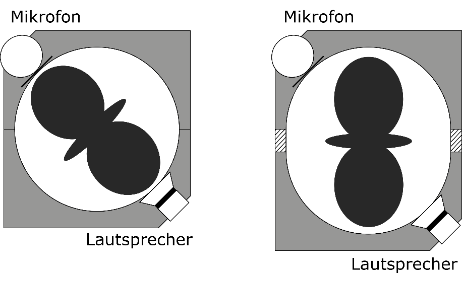
\includegraphics[width=0.7\textwidth]{Bilder/ressym.png}
        \caption{Aufbau zur Aufhebung der Entartung und resultierende 
        Ausrichtung der stehenden Wellen. \cite{anleitung15}}
    \hfill
    \label{fig:t1}
\end{figure}
